%!TEX root = ../../thesis.tex

\graphicspath{{Chapters/appendix_bonsai/figures/}}

\subsection{Optimizations}
While the extensive usage of pruners through our supernet means there is a tremendous amount of architectural flexibility,
it does mean that some of the largest number of function calls of any one component within the network come from the pruner
calculations, and as such need to be made as efficient as possible. To optimize the pruner function requires
creating gradient-safe tensor versions of equations~\ref{eq:gate} and~\ref{eq:saw} with the minimum number of function calls.
By \textit{gradient-safe}, I refer to ensuring that the gradient of our proposed tensor operation has the expected gradient
throughout the reasonable working range of the operation.  This was in particular an issue with two of my early
implementations of the gate:
\begin{align}
	G(w)_1 &=  \frac{w}{2|w|} + \frac{1}{2} \label{eq:absgate}\\
	G(w)_2 &= \texttt{sigmoid}(Mw)  \label{eq:siggate}
\end{align}

\begin{figure}[ht]
	\centering
	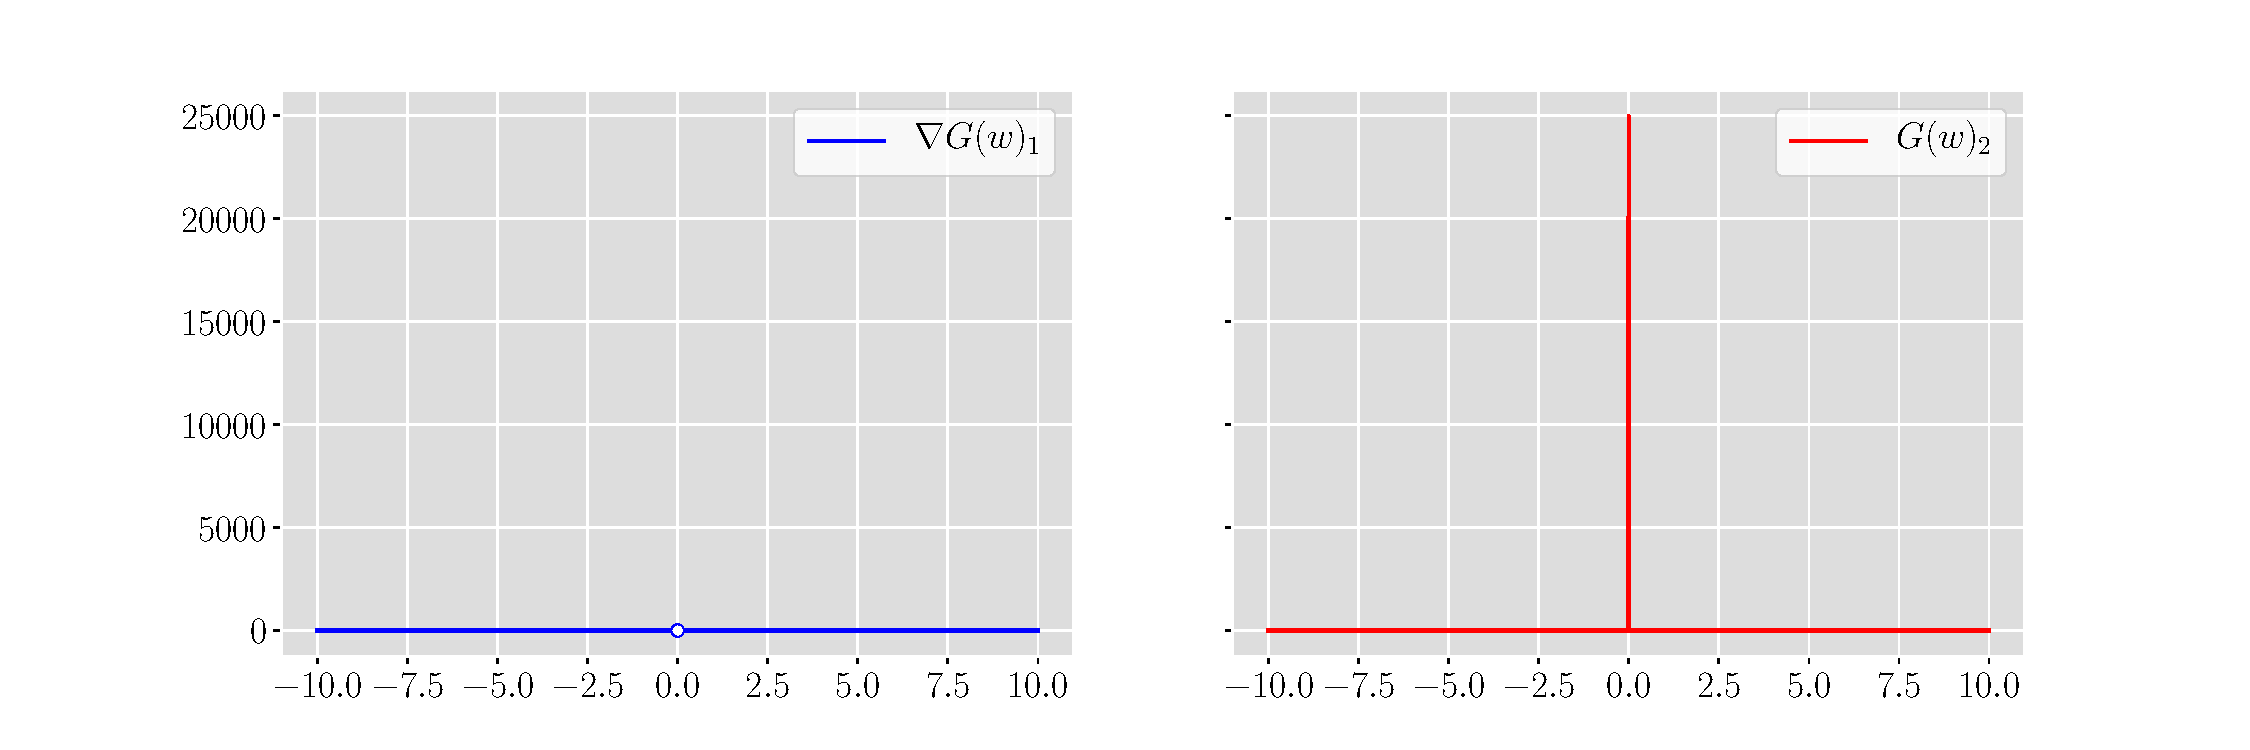
\includegraphics[width=\textwidth]{flawed_gate}
	\caption{Comparison of the gradient with respect to $w$ of the two gradient-unsafe gate implementations given in
	equations~\ref{eq:absgate} and~\ref{eq:siggate}.}
	\label{fig:badgates}
\end{figure}

The first gate implementation described in equation~\ref{eq:absgate} was designed because it performed gating through
exclusively mathematical means, without need for piecewise or boolean logic. This was because I was not entirely sure of
how boolean operations
worked in respect to gradient calculation in Torch, so this implementation entirely avoided the issue. It does manage
to provide the correct values over the majority of the range of $w$, but it and its gradient is undefined at $w=0$.
In the rare occurrences where SGD would cause a pruner to take on a weight of exactly 0, this gate function would cause
the pruner to output \texttt{nan} values. This then causes every operation subsequent to this pruner in the network to also
output \texttt{nan}s, which then spread to the rest of the network in backpropagation. This exemplifies the danger of gradient-unsafe operations, as a single \texttt{nan} output or gradient
will rapidly corrupt an entire model.

To try and fix the issues with the absolute value gate, I tried the second candidate gate function
equation~\ref{eq:siggate}. The principle behind this design was to again use entirely non-piecewise and non-boolean means
to approximate the gate, using the same value of $M$ from the saw function to drastically steepen and sharpen a sigmoid
function. Functionally, this works near identically to a gate, but the problem lies in its gradient in the area
close to 0. As seen in Figure \ref{fig:badgates}, the steepened sigmoid has a tremendously large gradient spike at zero.
If we were to try to update the weight at such a spike via the SGD equation
$\Delta \mathbf{w}_t = - \eta \nabla \mathit{G}(\mathbf{w}_t)$, we would end up changing the weight by a massive amount.
The issue with this is that the ``interesting" range of the pruner is in the domain immediately around 0, this is the decision
boundary between preserving and pruning a connection. Ideally, this decision is relatively harmless to experiment with; the model
should be able to switch an edge on or off, determine if that change is beneficial, and revert the change if desired without
lasting consequences. Indeed, we notice that pruners almost always exhibit this ``toe dipping"  behavior, moving across
the decision boundary for very short intervals, repeatedly experimenting with whether or not to preserve a particular edge.

However, the steep sigmoid gate function's gradient spike means that as soon as a pruner reaches this decision boundary
the weight will skyrocket to some massively negative or positive value.
The gradient at this extreme value will be be several orders of magnitude smaller than the gradient spike,
meaning the pruner weight will take a significant amount of time to return to the decision boundary, if ever. With such a gradient spike, moving a pruner weight across the decision boundary is permanent in practice. Since every pruner in the model will likely
cross the decision boundary at some point as part of the ``toe dipping", pruning becomes a purely stochastic decision, a
random sampling of whichever pruners happened to hit the boundary first.

Through experimenting with a variety of gate implementations, I eventually settled on the following as having the minimum
number of underlying CUDA function calls and fastest execution time while remaining gradient safe:
\begin{align}
	G(w) &=  \texttt{boolean}(w > 0)
\end{align}
Since Torch computes gradients discretely, the computed gradient for all values of $w$ is uniformly 0;
it is impossible to sample a point that actually lies on the discontinuity of this particular function.

Next, we look to the saw implementation. This needs to oscillate imperceptibly around 0 with a constant gradient of 1,
while remaining strictly greater than 0. This second criteria is important to make sure we never flip the sign of the incoming tensor,
such as to ensure the pruner is as transparent as possible. The first implementation was identical to the equation
given in the original paper:
\begin{align}
	S(w) &= \frac{M w - \lfloor M w \rfloor}{M} \label{eq:rawsaw}
\end{align}

This implementation is gradient-safe and performs mathematically correctly. However, it consists of four discrete operations
(the multiplication of $M$ by $w$, the floor operation, the subtraction, and the final division), which entails four total
tensor initializations to store the intermediate calculations of the operation as well as a high number of CUDA function calls.
Like previously stated, the saw is in the absolute innermost loop of the model execution, and thus is a crucial area for optimization.
As such, I designed the following optimized implementation:
\begin{align}
	S(w) &= w\Mod{\frac{1}{M}} \label{eq:optsaw}
\end{align}

This is mathematically identical to the original raw implementation, but makes use of the in-built CUDA function for computing
moduli called \texttt{remainder}. The theoretical advantage here is that \texttt{remainder} is CUDA-native, meaning its forward
and backward calculation are already optimised on a compiler level. The function only involves a single CUDA operation,
meaning there is only a single new tensor that needs to be initialized which should save some VRAM space compared to the
previous implementation. Additionally, since $\frac{1}{M}$ is constant throughout the lifespan of the pruner it
can be precomputed at initialization, further reducing the runtime. Table~\ref{tab:saw_implementations}
compares the performance of the two implementations:

\begin{table}[h]
\begin{center}
\begin{tabular}{c|c|c|c|c}
& & \multicolumn{2}{c|}{Runtime per 100 calls, ms} &  \\
Saw & CUDA Functions & Forward & Forward+Backward & VRAM\\
		  \hline
Raw		& 2 mul, 2 floor, 1 sub, 4 tensor init & 13.3 & 129.1 & 1200 Kb\\
Optimized     & 1 remainder, 1 tensor init & 2.8 & 18.3 & 100 Kb\\
\end{tabular}
\end{center}
\caption{Comparison of raw and optimized saw implementations.}
\label{tab:saw_implementations}
\end{table}

Checking runtime across both forward and forward-backward use cases is very important, specifically to check that
any performance advantage is present across both use cases. While only checking the forward pass is
the easier test to perform, the forward-backward use case is much more representative of the real-world application of any
particular operation. This is due to heavy reliance on the backwards operation during SGD training, and the cost
of the backwards operation being entirely independent to the cost of the forward operation. There are many times where
I've compared two candidate functions and found one to be faster than the other in the forward use case,
but its backward operation being orders of magnitude slower and thus completely cancelling out the forward advantage.
Operations like tensor indexing and the \texttt{sign} function are two such examples of these deceptive functions.
The remainder operation thankfully does not exhibit such deceptiveness, with results showing that the optimized saw runs
around 7 times faster than the raw saw in both use-cases. Furthermore, the need to only initialize a single tensor for
the optimized saw results in a VRAM savings of 1200\% compared to the raw saw.

In its original implementation, the addition of pruners to a model doubled its runtime. This meant that I focused a lot
of efforts in minimizing the amount of epochs that a model spent with active pruners, typically by performing intense
pruning in the first few epochs after a model reached its full size. However, as later results in
Section~\ref{sect:supernetevaluation} will show, the presence of pruners throughout training can highly benefit a model's
performance. With the new pruner implementations there is little-to-no overhead when including pruners into the model, which
means their preservation throughout pruning is relatively painless. This lets the pruner performance gains be realized
without compromising the search or train time of the models.


Another area for optimization occurs within the model nodes. The purpose of nodes within BonsaiNet are to sum
together all tensors that arrive at that node, and there are a few ways to perform this operation. As an example here,
we'll imagine a node that has three input edges, each with a number of component operations. The original way that
this node's output would be calculated was as follows, making some simplifications for clarity but preserving general
mechanics:

\begin{Verbatim}
	edge0_output = batch_norm(sum(edge0_ops))
	edge1_output = batch_norm(sum(edge1_ops))
	...
	edgeN_output = batch_norm(sum(edgeN_ops))
	node_input  = [edge0_output, edge1_output, ..., edgeN_output]
	node_output = batch_norm(sum(node_inputs))
\end{Verbatim}

Each edge is a self-contained unit in this construction; within the edge, the output of each component
operation is summed together, then batch normalized. This first batch normalization is the one as described in
Section~\ref{sect:pruner_batchnorm}. The node receives a number of edge outputs as its inputs,
then sums them together and batch normalizes the result to prevent the sum from getting too large. Due to the two
stage batch normalization, the output distribution of each edge is evenly balanced in the node input. This means that a
major change to any individual edge configuration has a significant effect on the the node output as a whole. Practically,
this serves to prevent any individual edge from pruning all of its component operations, presumably because the stepwise
difference between `only one operation on' and `all operations off' causes such a large downstream effect as to be
entirely unfeasible. Putting that detail aside momentarily, the first obvious performance optimization to make is to
combine the edge and node sums-batch normalization operations together:

\begin{Verbatim}
	edge0_output = [edge0_ops]
	edge1_output = [edge1_ops]
	...
	edgeN_output = [edgeN_ops]
	node_input  = concat(edge0_output, edge1_output, ..., edgeN_output)
	node_output = batch_norm(sum(node_input))
\end{Verbatim}

Here, each edge simply passes the outputs of its component operations out as a list. The node concatenates the output lists
from each of its inbound edges, and then sums all of them together at once. Finally, the sum of all inbound operations
to a node is batch normalized. While this is not mathematically identical to the first implementation, it performs the
same practical function: combine all the operations that arrive at a node, and ensure that they are normalized before they
pass downstream. The main difference is that normalization only occurs once here, meaning that each operation within each
of the edges can have varying distributions and contributions to the node input. Interestingly, models in this configuration
have no problem selecting for zero-operation edges, as a single edge moving from `only one operation on' and `all operations off'
changes only one of many components of the final node output sum.

The final performance gain comes from a seemingly strange discrepancy when benchmarking the function calls performed in the
above implementation. In the final summation \texttt{sum(node\_inputs)}, Torch calls a number of addition
operations and tensor allocations equal to the length of the \texttt{node\_inputs} list. However, one would assume when adding a list of $n$ numbers together,
only $n-1$ sums need to be computed:

\begin{center}
\begin{tabular}{ccccc}
$\text{sum}([a,b,c])$   & = & $a + b + c$ &\textrightarrow& 2 sums\\
$\text{sum}([a,b,c,d])$ & = & $a + b + c + d$ &\textrightarrow&3 sums
\end{tabular}
\end{center}

\noindent The issue occurring here is due to the Python $\texttt{sum}$ function's default \texttt{start}
argument of 0, which sets the initial value of the running sum performed by the function. This means the actual computation
performed is:

\begin{center}
\begin{tabular}{ccccc}
$\text{sum}([a,b,c])$   & = & $a + b + c + 0$ &=& 3 sums\\
$\text{sum}([a,b,c,d])$ & = & $a + b + c + d + 0$ &=&4 sums
\end{tabular}
\end{center}

\noindent In our case, 0 would be added to the first tensor in the node input before the rest of the sum
would be calculated. The fact that the default argument is an raw Python integer that is added to a floating point
tensor gives this a massive function call overhead in Torch; summing a list of length
$n$ is this way requires $n$ adds, $n+1$ tensor initializations, 1 tensor copy, and 1 tensor cast for the forward pass alone.
This can be remedying by instead setting the \texttt{start} argument to be the first item in our node input list,
and summing over the remaining elements:

\begin{Verbatim}
	edge0_output = [edge0_ops]
	edge1_output = [edge1_ops]
	...
	edgeN_output = [edgeN_ops]
	node_input  = concat(edge0_output, edge1_output, ..., edgeN_output)
	node_output = batch_norm(sum(node_input[1:], start=node_input[0]))
\end{Verbatim}

\noindent This reduces the function calls for that sum to what we would expect; $n-1$ adds and $n-1$ tensor
initializations. This has the effect of reducing the total forward-backward time of each summation by around 16\% and
reducing the memory allocation cost by 42\%.